\documentclass[a4paper,10pt,notitlepage,pdftex,headsepline]{scrartcl}

\usepackage{geometry}
\geometry{left=2cm}
\geometry{right=2cm}
\geometry{top=1cm}
\geometry{bottom=1cm}

\usepackage{cmap} % чтобы работал поиск по PDF
\usepackage[utf8]{inputenc}
\usepackage[russian]{babel}
\usepackage[T2A]{fontenc}

\usepackage{textcase}
\usepackage[pdftex]{graphicx}

\pdfcompresslevel=9 % сжимать PDF
\usepackage{pdflscape} % для возможности альбомного размещения некоторых страниц
\usepackage[pdftex]{hyperref}
% настройка ссылок в оглавлении для pdf формата
\hypersetup{
	unicode=true,
    pdftitle={},
    pdfauthor={Погода Михаил},
    pdfcreator={pdflatex},
    pdfsubject={},
    pdfborder    = {0 0 0},
    bookmarksopen,
    bookmarksnumbered,
    bookmarksopenlevel = 2,
    pdfkeywords={},
    colorlinks=true, % установка цвета ссылок в оглавлении
    citecolor=black, 
    filecolor=black,
    linkcolor=black,
    urlcolor=blue
}

\usepackage{amsmath}
\usepackage{amssymb}
\usepackage{moreverb}
\author{Michael Pogoda}
\title{plab311}
\date{\today}

\begin{document}
\begin{enumerate}
\item Монохрометр-спектроскоп УМ-2 --- прилад для вимірювання довжини хвиль спектр. ліній.

Діапазон: $3800\dots10000$ А.
\item Окремі лінії у спектрах атомів можно об’єднати у групи ліній, що називаються серіями.
У 1885 році Бальмер помітив, що частоти ліній у видимій частині спектра водню можна виразити формулою
$$\nu_{m_2} = R\left(\frac{1}{r^2} - \frac{1}{m^2}\right), m = 3,4,5\dots$$

Пізніше були відкриті нові серії ліній.
*** формула показує, що кожна з частот є різницею двох величин, які залежать від цілого числа.
\item Кожному атому можна співставити *** таблицю чисел, або спетральних ***.
При цьому усі частоти випромінюваються, що спостерігаються, можна отримати, комбінуючи різні пари ***.
Це правило називається принципом Різберга-***
$$\nu_{m_n} = T\left(n\right) - T\left(m\right), T\left(m\right) = \frac{R}{m^2}$$
\item Постулати Бора:
\begin{itemize}
\item Атомна система може перебувати тільки в особливих стаціонарних або квантових станах, кожному з яких відповідає повна енергія $E_n$.
У стаціонарному стані атом енергію не випромінює.
\item Перехід атому зі стаціонарного стану в інший супроводжується випромінюванням чи поглинанням фотонів, енергію яких $h\nu$ виражається за формулою
$$ h\nu_K = E_K - E_h$$
\item Радіус $r_n$ стаціонарних станів задовільняє умові:
$$m v_n r_n = n\frac{h}{2\pi} = n\hbar$$
Спектральні терми мають певний фізичний сенс, котрий є пов’язаниним з енергією стаціонарних станів атома, а комбінуючи принцип Рітуя стає природним *** першого *** Бору.
\end{itemize}
\item б) $E_n = \frac{z^2 m_e e^4}{32\pi^2\varepsilon_0^2 \hbar^2} \cdot \frac{1}{n^2}$, де $z$ --- кількість протонів, $n\to\inf, E\to 0$

Енергія першої орбіти $E = -13,6$ еВ і є енергією ***.
\item Відповідно до квантової теорії під час перехода атома зі стану $E_n$ у стан $E_m$ випромінюється фотон з енергією $\hbar \omega_{nm} = E_n-E_m$, тому
$$E_n = - \frac{me^4}{32\pi^2\varepsilon_0^2\hbar^2} \cdot \frac{1}{n^2}$$
У спектр атому --- дискретні частоти
$$\omega_{nm} = \frac{me^4}{32\pi^2\varepsilon_0^2\hbar^2} \left(\frac{1}{m^2} - \frac{1}{n^2}\right) = R\left(\frac{1}{m^2} - \frac{1}{n^2}\right)$$
$R$ --- стала Різберга
\item текст

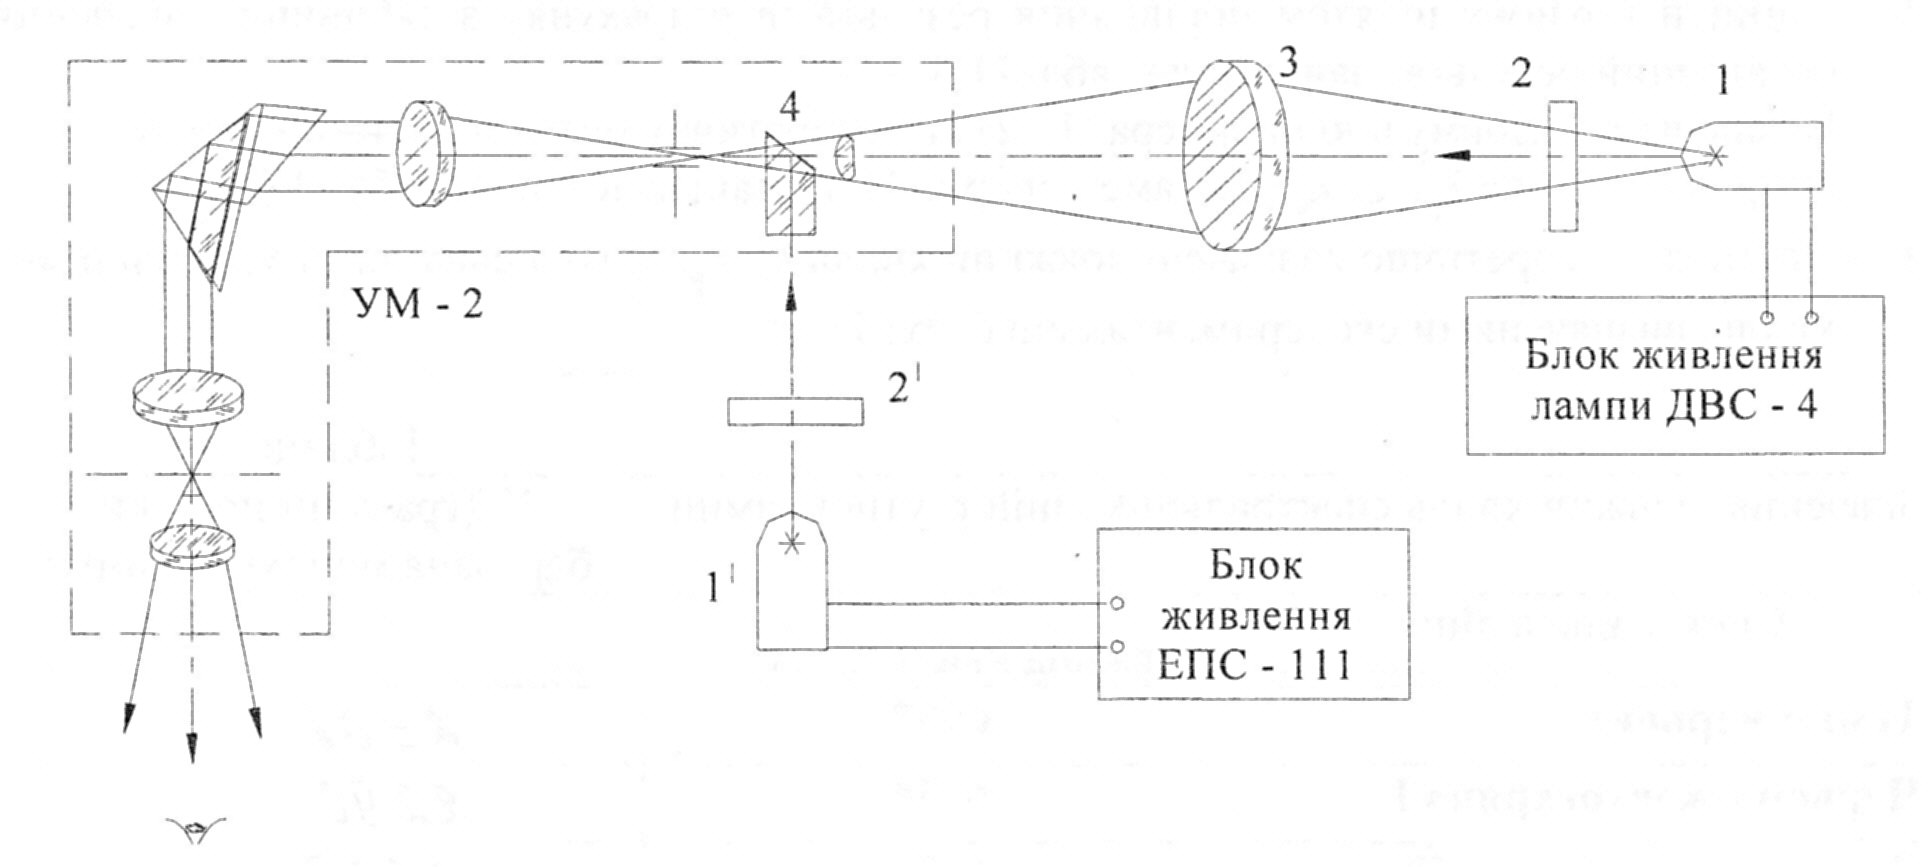
\includegraphics{img.jpg}
\item Принцип відповідності --- одне з положень ко*** інтерпритації квантової механіки, яка вимогає щоб при збільшенні розмірів фізичного спек* її квантової властивості переходити ***.
\end{enumerate}
\end{document}